\documentclass[a4paper,12pt]{article}
\usepackage[a4paper,top=1.3cm,bottom=2cm,left=1cm,right=1cm,marginparwidth=0.75cm]{geometry}

% Пакеты
\usepackage{mathtext} 
\usepackage{setspace}
\usepackage{tabularx}
\usepackage{cmap}
\usepackage{longtable}
\usepackage{icomma}
\usepackage{euscript}
\usepackage{float}
\usepackage{cutwin}
\usepackage{mathrsfs}
\usepackage{adjustbox}
\usepackage{dashbox}
\usepackage[normalem]{ulem}
\usepackage[T1,T2A]{fontenc}			
\usepackage[utf8]{inputenc}                 %!  закрепляет кодировку utf8
\usepackage[english,russian]{babel}         %!  подключает русский и английский
\usepackage[babel=true]{microtype}
\RequirePackage[T1]{fontenc}
%математические шрифты:
\usepackage{amsmath,amsfonts,amssymb,amsthm,mathrsfs,mathtools} 
%!\usepackage[colorlinks, linkcolor = purple]{hyperref}      %!  оглавление для панели навигации по PDF-документу + гиперссылки
\usepackage{xcolor}                         %!  добавляет цвета
\usepackage{enumitem}                       %!  задание макета перечня.
\usepackage{xpatch}                         %?  работа с renewcommand и макросами              
\usepackage{cancel}                         %   зачёкивания текста (!!!) для slash-нотации использовать \usepackage{slashed}!!
\usepackage{upgreek}                        %   заглавные греческие буквы
\usepackage{lipsum}                         %?  для вставки кучи текста при форматировании
\usepackage[version=4]{mhchem}              %   химические формулы
\usepackage{multirow}                       %   объединение строк в матрицах
\usepackage{stackengine}                    %   stack символов
\usepackage{tikz}                           %!  рисунки
\usetikzlibrary{positioning}                %?  библиотека для тикза 
\usepackage{titletoc}                       %!  форматирование содержания и заголовков
\usepackage{titlesec}                       %!  форматирование содержания и заголовков
\usepackage{wrapfig}                        %   обтекание таблиц и рисунков
\usepackage{chngcntr}                       %!  для setcounter
\usepackage{fancyhdr}                       %!  для колонтитулов
\usepackage{makecell}                       %?  матрицы с разными выравниваниями и т.п
\usepackage{indentfirst}                    %   добавить indent перед первым 
\usepackage{tocloft}                        %?  изменение названий глав и разделов                       
\usepackage{soul}                           %   типографические примочки, типо зачёркивания и подчёркивания
\usepackage[stable]{footmisc}               %?  продвинутые сноски
\usepackage{subfig}                         %   несколько картинок рядом
%  задаёт поля страниц

% pgf plots
% \usepackage{pgfplots}
% \pgfplotsset{compat=1.17}

\mathtoolsset{showonlyrefs=true}

%Обозначения теорем и т.п
\theoremstyle{definition}
\newtheorem*{definition}{Определение}
\newtheorem{statement}{Предложение}[section]
\newtheorem{lemma}{Лемма}[section]
\newtheorem{theorem}{Теорема}[section]
\newtheorem*{theoremn}{Теорема}
\newtheorem*{corollary}{Следствие}
\newtheorem*{example}{Пример}
\newtheorem*{note}{Замечание}
\newtheorem*{problem}{Задача}

%Шарабара для содержания и внешнего вида нумерации
\counterwithout{footnote}{section}\DeclareRobustCommand{\divby}{%
	\mathrel{\text{\vbox{\baselineskip.65ex\lineskiplimit0pt\hbox{.}\hbox{.}\hbox{.}}}}%
}



%Толерантный квадратик чтд
%\makeatletter \renewenvironment{proof}[1][\proofname]{\par\pushQED{\qed}\normalfont\topsep6\p@\@plus6\p@\relax\trivlist\item[\hskip\labelsep\bfseries#1\@addpunct{.}]\ignorespaces}{\popQED\endtrivlist\@endpefalse} \makeatother
%\renewcommand\qedsymbol{$\squareulblack$}
%\newcommand{\usubseteq}{\mathbin{\rotatebox[origin=c]{90}{$\subset$}}}
%\DeclareFontEncoding{LS2}{}{\noaccents@}
%\DeclareFontSubstitution{LS2}{stix}{m}{n}
%\DeclareSymbolFont{arrows3}{LS2}{stixtt}{m}{n}
%\DeclareMathSymbol{\squareulblack}{\mathord}{arrows3}{"88}

%Разные операторы и символы
\newcommand{\dotpr}[2]{\bra{#1}\ket{#2}}
\let\AA\relax
%\let\oldvarphi\phi %оно делает так, что \phi становится правильным фи
%\let\phi\varphi
%\let\varphi\oldvarphi
\let\emptyset\varnothing
\DeclareMathOperator*{\esssup}{ess sup}
\DeclareMathOperator*{\ord}{ord}
\DeclareMathOperator*{\supp}{supp}
\DeclareMathOperator*{\pr}{pr}
\DeclareMathOperator*{\Ker}{Ker}
\DeclareMathOperator*{\Vol}{Vol}
\DeclareMathOperator*{\rg}{rk}
\DeclareMathOperator*{\Ima}{Im}
\DeclareMathOperator*{\Alt}{Alt}
\DeclareMathOperator*{\Sym}{Sym}
\newcommand{\eqdef}{\stackrel{\text{\tiny{def}}}{=}}
\newcommand{\pp}{\partial}
\newcommand{\AA}{\mathcal{A}}
\newcommand{\BB}{\mathcal{B}}
\newcommand{\MM}{\mathbb{M}}
\newcommand{\NN}{\mathbb{N}}
\newcommand{\ZZ}{\mathbb{Z}}
\newcommand{\QQ}{\mathbb{Q}}
\newcommand{\RR}{\mathbb{R}}
\newcommand{\CC}{\mathbb{C}}
\newcommand{\FFF}{\mathbb{F}}
\newcommand{\DD}{\mathcal{D}}
\newcommand{\FF}{\mathcal{F}}
\newcommand{\sS}{\mathcal{S}}
\newcommand*\circled[1]{\tikz[baseline=(char.base)]{
		\node[shape=circle,draw,inner sep=2pt] (char) {#1};}}


\title{Получение и измерение вакуума (2.3.1)}
\author{Павлушкин Вячеслав}
\date{\today}


\begin{document}
	\maketitle
	
	\section{Введение}
	\noindent\textbf{Цель работы:} 1) измерение объемов форвакуумной и высоковакуумной частей установки; 2) определение скорости откачки системы в стационарном режиме, а также по ухудшению и улучшению вакуума.\\
	\bigskip
	
	\noindent\textbf{В работе используются:} вакуумная установка с манометрами: масляным, термопарным и ионизационным.
	
	\section{Экспериментальна установка}
	
	\begin{figure}[h!]
		\centering
		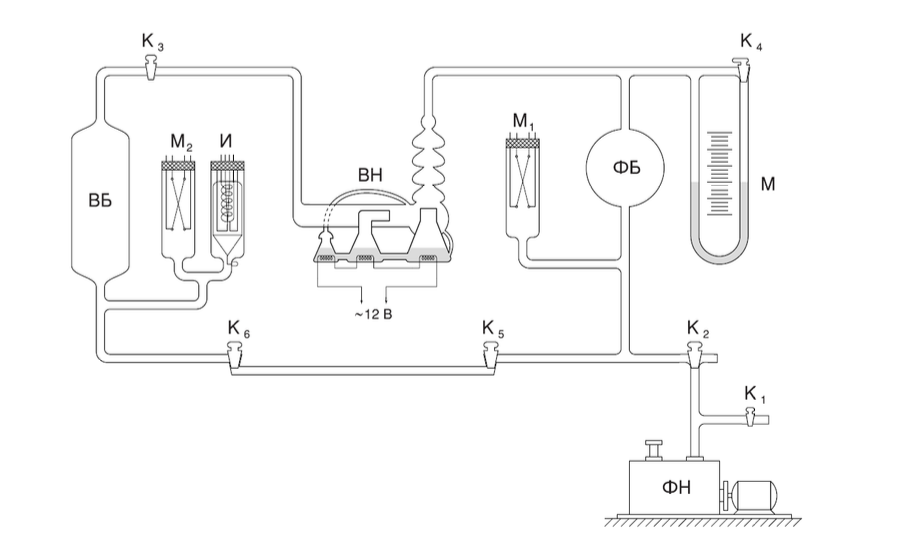
\includegraphics[scale=0.53]{facility.jpg}
		\caption{Схема экспериментальной установки}
		\label{facility}
	\end{figure}

	Установка изготовлена из стекла,
	и состоит из форвакуумного баллона (ФБ), высоковакуумного диффузионного насоса (ВН), высоковакуумного баллона (ВБ), масляного (М) и ионизационного (И) манометров, термопарных манометров ($\text{М}_1$ и $\text{М}_2$), форвакуумного насоса (ФН) и соединительных кранов ($\text{K}_1, \text{K}_2,\; \ldots \;\text{K}_6$) (Рис. \ref{facility}). Кроме того, в состав установки входят: реостат и амперметр для регулирования тока нагревателя диффузионного насоса.
	
	\begin{wrapfigure}{l}{6cm}
		\centering
		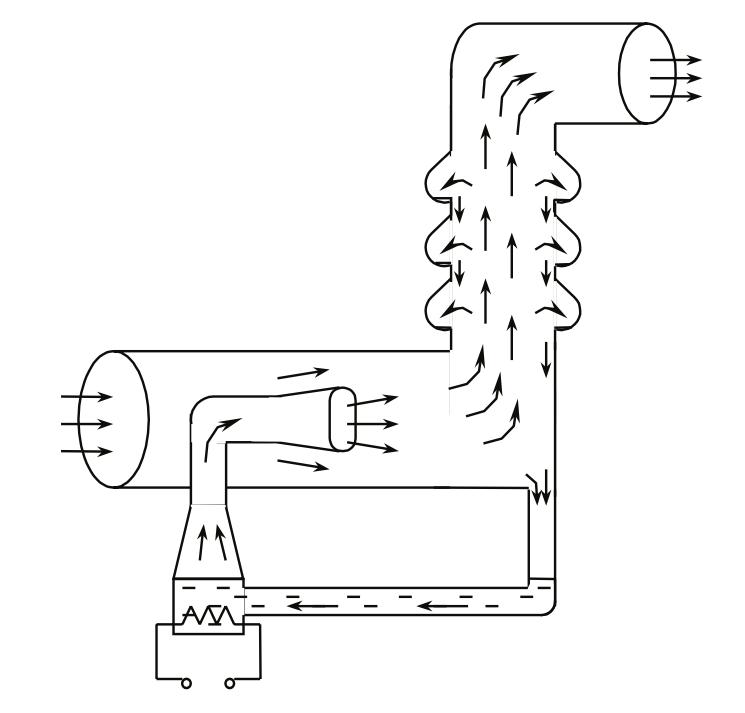
\includegraphics[width=1\linewidth]{pump}
		\caption{Схема работы высоковакуумного насоса}\label{pump}
	\end{wrapfigure}

	Устройство масляного диффузионного насоса схематически показано на Рис. \ref{pump} (в лабораторной установке используется несколько откачивающих ступеней). Масло, налитое в сосуд, подогревается электрической печкой. Пары масла поднимаются по трубе и вырываются из сопла. Струя паров увлекает молекулы газа, которые поступают из откачиваемого сосуда через трубку. Дальше смесь попадает в вертикальную трубу. Здесь масло осаждается на стенках трубы и маслосборников после чего стекает вниз, а оставшийся газ откачивается форвакуумным насосом. 
	
	\section{Теоретические сведения}
	\subsection{Процесс откачки}
	
	Опишем процесс откачки математически: 
	Пусть W --- объем газа, удаляемого из сосуда при данном давлении за единицу времени, $Q_i$ для различных значений $i$ обозначим различные притоки газа в сосуд (в единицах $PV$), такие как течи извне $Q_\text{и}$, десорбция с поверхностей внутри сосуда $Q_\text{д}$, обратный ток через насос $Q_\text{н}$. Тогда имеем:
	\begin{equation}
		-VdP = \left(PW - \sum Q_i\right)dt
	\end{equation}
	При достижении предельного вакуума устанавливается $P_{\text{пр}}$, и $dP = 0$. В таком случае:
	\begin{equation}
		W = \biggl( \sum Q_i \biggr)\bigg/ P_{\text{пр}}
	\end{equation}
	Поскольку обычно $Q_\text{и}$ постоянно, а $Q_\text{н}$ и $Q_\text{д}$ слабо зависят от времени, также считая постоянной W, можем проинтегрировать (1) и получить:
	\begin{equation}
		P - P_{\text{пр}} = (P_0 - P_{\text{пр}})\exp\left(-\frac{W}{V}t\right)
		\label{exp}
	\end{equation}
	Полная скорость откачки $W$, собственная скорость откачки насоса $W_{\text{н}}$ и проводимости элементов системы $C_1, C_2,\;\ldots$ соотносятся согласно формуле (4), и это учтено в конструкции установки.
	\begin{equation}
		\frac{1}{W} = \frac{1}{W_\text{н}} + \frac{1}{C_1} + \frac{1}{C_2} + \ldots
	\end{equation}
	
	\subsection{Течение газа через трубу}
	
	Характер течения газа существенно зависит от соотношения между размерами системы и длиной свободного пробега молекул. При атмосферном и форвакуумном давлениях  длина свободного пробега меньше диаметра трубок, и течение газа определяется его вязкостью, т.е. взаимодействием молекул. При переходе к высокому вакууму столкновения молекул между собой начинают играть меньшую роль, чем соударения со стенками.
	
	Для количества газа, протекающего через трубу длины $l$ и радиуса $r$ в условиях высокого вакуума, справедлива формула:
	\begin{equation}
		\frac{d(PV)}{dt} = \frac{4}{3}r^3\sqrt{\frac{2\pi RT}{\mu}}\cdot\frac{P_2 - P_1}{l}
	\end{equation}
	Если труба соединяет установку с насосом, то давлением $P_1$ у его конца можно пренебречь. Давление в сосуде $P = P_2$. Тогда пропускная способность трубы:
	\begin{equation}
		C_\text{тр} = \left(\frac{dV}{dt}\right)_\text{тр} = \frac{4r^3}{3l}\sqrt{\frac{2\pi RT}{\mu}}
		\label{ty}
	\end{equation}

	\section{Ход работы}
	
	\subsection{Определение объемов форвакуумной и высоковакуумной частей установки}
	
	\begin{enumerate}
	
	\item Перед началом работы проверим, что все краны приведены в правильное положение. 
	
	\item Запустим воздух в систему (для этого нужно открыть кран $К_2$  и подождать пару минут пока воздух заполнит установку). 
	
	\item Запустим форвакуумный насос, чтобы он откачал воздух из установки. 
	
	Пронаблюдаем за тем, как давление в установке уменьшается и продолжим откачку до момента, пока давление не будет порядка $ 10^{-2}~торр$.
	
	\item Отсоединим установку от форвакуумного насоса, а затем объем, заключенный в кранах и капиллярах форвакуумной части, откроем на всю форвакуумную часть. Тогда давление изменится
	
	\item Запишем показания масляного манометра, а именно высоту масла в обоих коленах: 
	\begin{align}
		h_1 = (34.9 \pm 0.1) ~см, && h_2 = (6.2 \pm 0.1) ~см,
	\end{align}
	\begin{align}
		\sigma_{\Delta h} = \sqrt{\sigma_{h1}^2 + \sigma_{h2}^2}\approx 1.6~\% & &
		\Delta h_{фв} = (28.7 \pm 0.5) ~см.
	\end{align}

	\item Зная объем "запертой"  части установки $V_{кап} = 50 ~см^3$ и используя соотношение $P_\text{А} V_{кап}=P_2 V_2$ вычислим объем форвакуумной части установки. При этом давление $P_1 = P_{атм} = (98.4 \pm 0.1) ~кПа$ $P_2 =   \rho_{масл} g \Delta h_{фв}$, а относительная погрешность полученного значения равна относительной погрешности величины $\Delta h_{фв} $:
	$$\varepsilon_V = \varepsilon_{P_1} \approx 1.6 ~\%.$$ и в результате имеем: 
	
	\begin{equation}
		V_{фв} = (1.97 \pm 0.03)~ л
	\end{equation}
	
	
	\item Проведем те же самые измерения с диффузионным насосом и получим объем установки, из которой вычитанием объема форвакуумной части получается объем высоковакуумной части. 
	\begin{align}
		h_3 = (29.8 \pm 0.1) ~см, && h_4 = (11.6 \pm 0.1) ~см,
	\end{align}
	\begin{align}
		\Delta h_{полн} = (18.2 \pm 0.2) ~см.
	\end{align}
	
	Погрешности высот определяются аналогично предыдущему пункту. Как и формула для полного объема установки, тогда:
	\begin{align}
		V_\text{полн} = \frac{P_\text{А}}{\rho g \Delta h_\text{полн}} V_{кап} \approx 3.11~л,&&
		\varepsilon_{V_{полн}} = \varepsilon_{\Delta h} \approx 1~\%.
	\end{align}

	В результате искомая величина равна:
	\begin{align}
		V_{вв} = V_{полн} - V_{фв} = 1.14~л, && \sigma_{V_{вв}} = \sqrt{\sigma_{V_{полн}}^2+ \sigma_{V_{фв}}^2} \approx 0.04~л,
	\end{align}
	\begin{align}
		V_{вв} = (1.14 \pm 0.04)~л.
	\end{align}
	
	\end{enumerate}

	\subsection{Получение высокого вакуума и измерение скорости откачки}
	
	\begin{enumerate}
		\setcounter{enumi}{7}
		
		\item Не выключая форвакуумного насоса убедимся в том, что в установке не осталось запертых объемов. 
		
		\item Откачав установку до давления порядка $ 10^{-2}~торр$, приступим к откачке ВБ с помощью диффузионного насоса. 
		
		
		\item С помощью термопарного манометра пронаблюдаем за тем, как идет откачка ВБ. Мы должны продолжать процесс откачки до тех пор, пока там не установится давление порядка $3 \cdot 10^{-4}~торр.$ При приближении давления к этой величине масло в диффузионном насосе закипит, поэтому подсчитаем количество капель, стекающих из сопла второй ступени диффузионного насоса: $$ N = 10 ~ капель.$$
		
		\item С помощью ионизационного манометра измерим значение предельного давления в системе со стороны высоковакуумной части: $$P_{пр} = (8.3 \pm 0.1)  \cdot 10^{-5} ~торр.$$
		
		
		\item Найдем скорость откачки по ухудшению и улучшению вакуума, для этого открывая и закрывая кран $К_3$ будем то подключать насос к объему, то отключать его, при этом на видео зафиксируем показания манометра от времени и построим графики необходимых  зависимостей (каких именно подробнее описано в соответствующих пунктах ниже), для которых определим коэффициенты наклона прямых и их погрешности (с помощью МНК).
		
		Для случая улучшения вакуума воспользуемся формулой \eqref{exp} и построим график зависимости $(ln(P-P_{пр}))$ от $t$. При построении такого графика из МНК получим коэффициент наклона --- $k$, с помощью которого можно найти $W = -kV_{вв}$. Построим эти графики (Рис. \ref{graph2}, \ref{graph3}, \ref{graph4}):
		\begin{figure}[h!]
			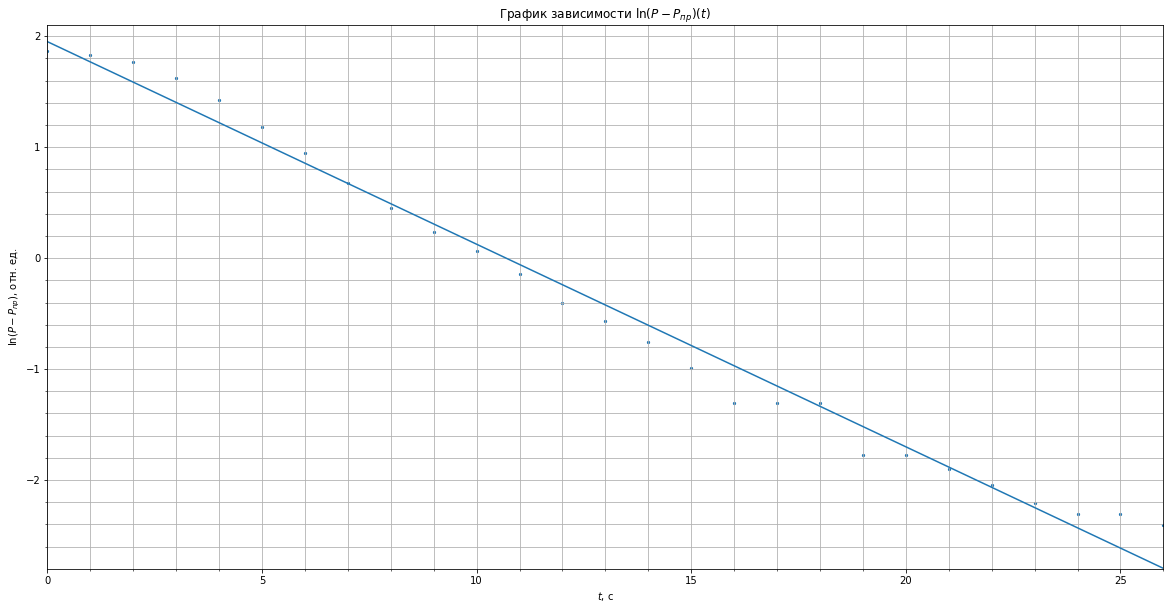
\includegraphics[scale=0.43]{graphdown2}
			\caption{Улучшение вакуума 1}
			\label{graph2}
		\end{figure}
		\bgroup
		\def\arraystretch{1.3}%
		\begin{table}[H]
			\begin{center}
				\begin{tabular}{|c|c|c|c|c|c|}
					\hline
					$k,~\frac{1}{с}$ & $\sigma_k^{сл},~\frac{1}{с}$ &$\sigma_k,~\frac{1}{с}$& $k_{ср},~\frac{1}{с}$ & $W,~\frac{л}{с}$ & $\sigma_W,~\frac{л}{с}$\\
					\hline
					-0.183& 0.004 & 0.02 & \multirow{3}{*}{-0.176}& \multirow{3}{*}{0.20}& \multirow{3}{*}{0.02}\\
					\cline{1-3}
					-0.173&0.004&0.02&&&\\
					\cline{1-3}
					-0.173&0.004&0.02&&&\\
					\hline
				\end{tabular}
			\end{center}
			\caption{Коэффициенты наклона при улучшении вакуума}
			\label{tab1}
		\end{table}
		\egroup
		\item Оценим величину потока газа  $Q_Н$. Для этого воспользуемся данными, полученными при ухудшении вакуума. А именно построим графики зависимости $P(t)$ и определим для них коэффициенты угла наклона прямой. Поскольку $V_{вв}dP = (Q_Д + Q_И) dt$ получим $(Q_Д + Q_И) = kV_{вв}$. По графикам получаем:
		\bgroup
		\def\arraystretch{1.3}%
		\begin{table}[h!]
			\begin{center}
				\begin{tabular}{|c|c|c|c|c|c|}
					\hline
					$k\cdot 10^{-6},~\frac{торр}{с}$ & $\sigma_k^{сл}\cdot 10^{-6},~\frac{торр}{с}$ &$\sigma_k\cdot^{-6},~\frac{торр}{с}$& $k_{ср}\cdot10^{-6},~\frac{торр}{с}$ & $Q_{д}+Q_{и},~торр\cdot\frac{л}{с}$ & $\sigma_{Q_{д}+Q_{и}},~торр\cdot\frac{л}{с}$\\
					\hline
					9.8& 0.1 & 0.15 & \multirow{4}{*}{9.8}& \multirow{4}{*}{$1.12\cdot10^{-5}$}& \multirow{4}{*}{$0.04\cdot10^{-5}$}\\
					\cline{1-3}
					10.0&0.1&0.15&&&\\
					\cline{1-3}
					10.0&0.1&0.15&&&\\
					\cline{1-3}
					9.5&0.1&0.14&&&\\
					\hline
				\end{tabular}
			\end{center}
			\caption{Коэффициенты наклона при ухудшении вакуума}
			\label{tab2}
		\end{table}
		\egroup
		\begin{figure}[h!]
			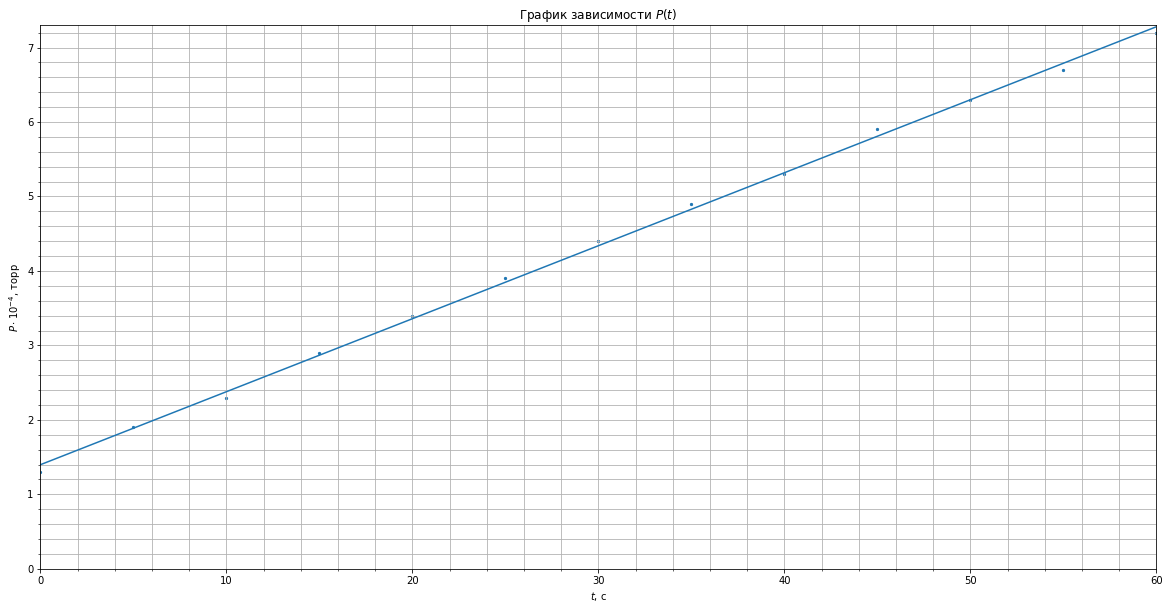
\includegraphics[scale=0.43]{graphup1}
			\caption{Ухудшение вакуума 1}
			\label{graphup1}
		\end{figure}
		Используя формулу $Q_Н = P_{пр}W - (Q_Д + Q_И)$, а значит $\varepsilon_{Q_Н} =  \sqrt{\varepsilon_{P_{пр}W}^2 + \varepsilon^2} \approx 10.4\%$ получим, что: $Q_Н = (5.4 \pm 0.08) \cdot 10^{-6} ~ торр \cdot л / с.$
		
		
		
		\item Оценим пропускную способность трубки по формуле (6):
		\begin{align}
			L = (10 \pm 1)~ см; &&   d = (0.8 \pm 0.1) ~ мм,
		\end{align}
		
		\begin{equation}
			C_{тр} = (2.1 \pm 0.1)~л / с.
		\end{equation}
		
		Погрешность $C_{тр}$  оценена как корень из суммы квадратов погрешностей длинны и диаметра (которые явным образом не указаны на установке, оценка довольно грубая).
		
		Скорость откачки по порядку сходится с пропускной способностью трубки, что означает -- эксперимент достаточно успешен.
		
		\item Введем в систему искусственную течь и запишем значение  установившегося при этом давления и давления $P_{фв}$: 
		
		\begin{align}
			P_{уст} = (1.2 \pm 0.1) \cdot 10^{-4} ~ торр. && P_{фв} = (1.6 \pm 0.1) \cdot 10^{-3} ~ торр.
		\end{align}
		
		
		\item Поскольку
		$$P_{пр} W = Q_1, \quad P_{уст} W = Q_1 + \frac{d(PV)_{кап}}{dt},$$
		то с учетом \eqref{ty}, получаем:
		\begin{equation}
			W = \frac{P_{фв}}{P_{уст}-P_{пр}}\frac{4r^3}{3L}\sqrt{\frac{2\pi RT}{\mu}} \approx 0.046~\frac{л}{с}
		\end{equation}
		
		(Поскольку давления померены с точностью не менее $10\%$, то можно учитывать погрешность, вносимую величиной $\frac{d(PV)_{кап}}{dt}$ относительная погрешность которой равна относительной погрешности $C_{тр}$, то есть составляет $5\%$)
		
		
		\item Следуя указаниям в методичке выключаем установку.
		
	\end{enumerate}
	
	\section{Вывод}
	\begin{itemize}
		\item Измерили объемы форвакуумной, высоковакуумной части установки, так же как и объем всей установки.
		
		\item Определили скорость откачки двумя способами.
		
		Возможными причинами расхождения полученных результатов на один порядок могло послужить изменение температуры, созданное нагреваемым масляным высоковакуумным насосом. Также возможна разница из-за принципа работы высоковакуумного насоса -- при уменьшении давления в нем, производительность начинает падать.
		
		\item Оценили поток газа, поступающего из насоса в откачиваемую систему.
		
		
		
		
	\end{itemize}
	
	\newpage
	
	\section{Приложение}
	
	\centering
	\begin{figure}[h!]
		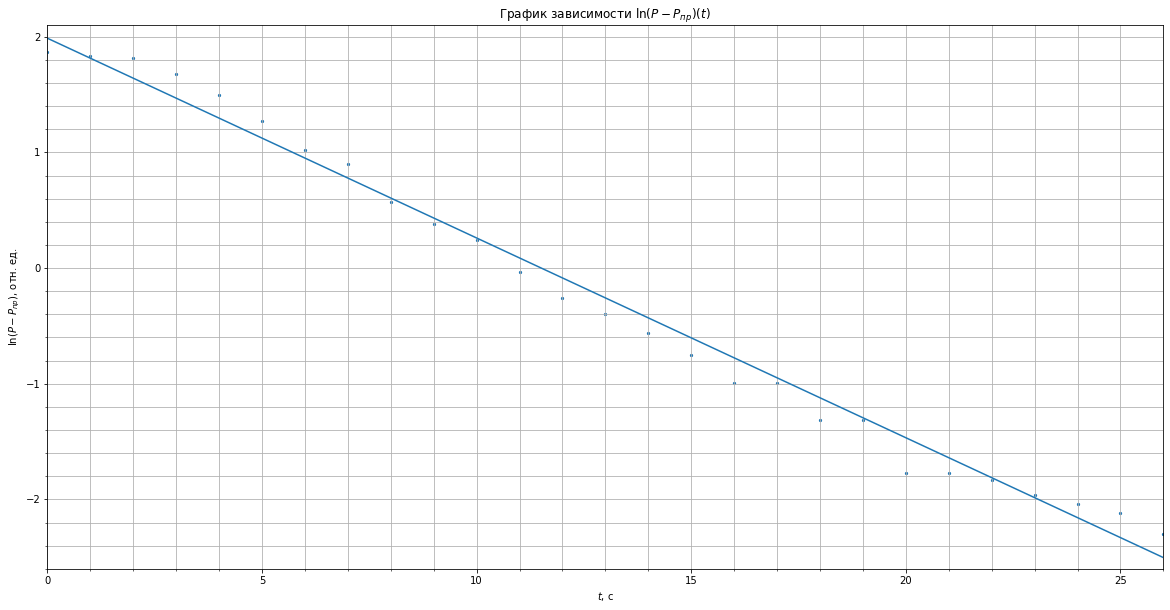
\includegraphics[scale=0.43]{graphdown3}
		\caption{Улучшение вакуума 2}
		\label{graph3}
	\end{figure}

	\begin{figure}[h!]
		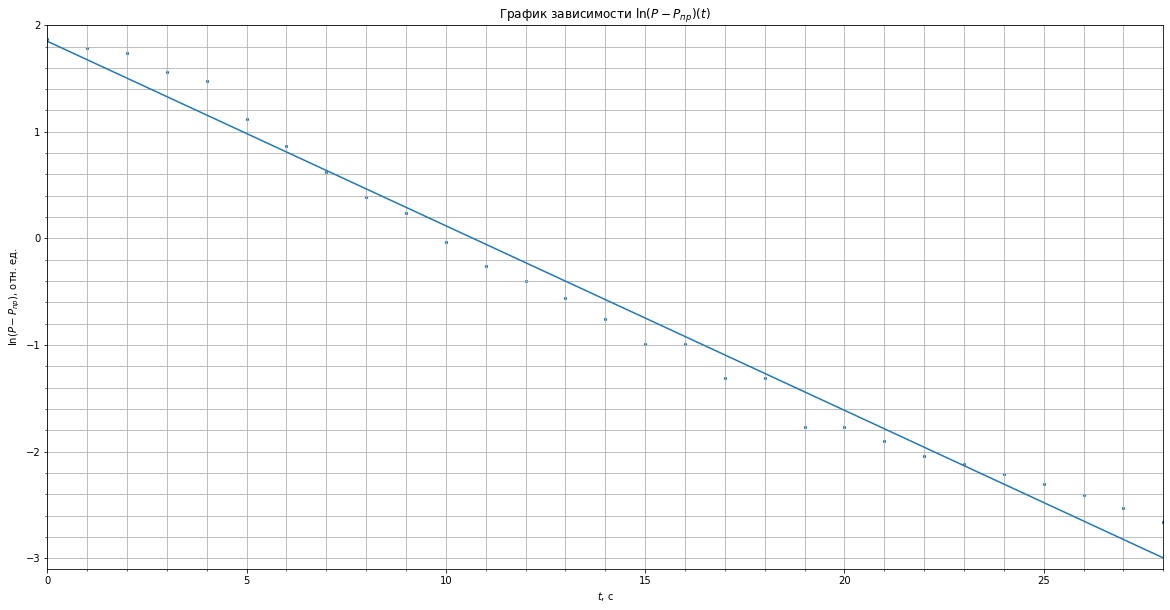
\includegraphics[scale=0.43]{graphdown4}
		\caption{Улучшение вакуума 3}
		\label{graph4}
	\end{figure}
	
	\begin{figure}[h!]
		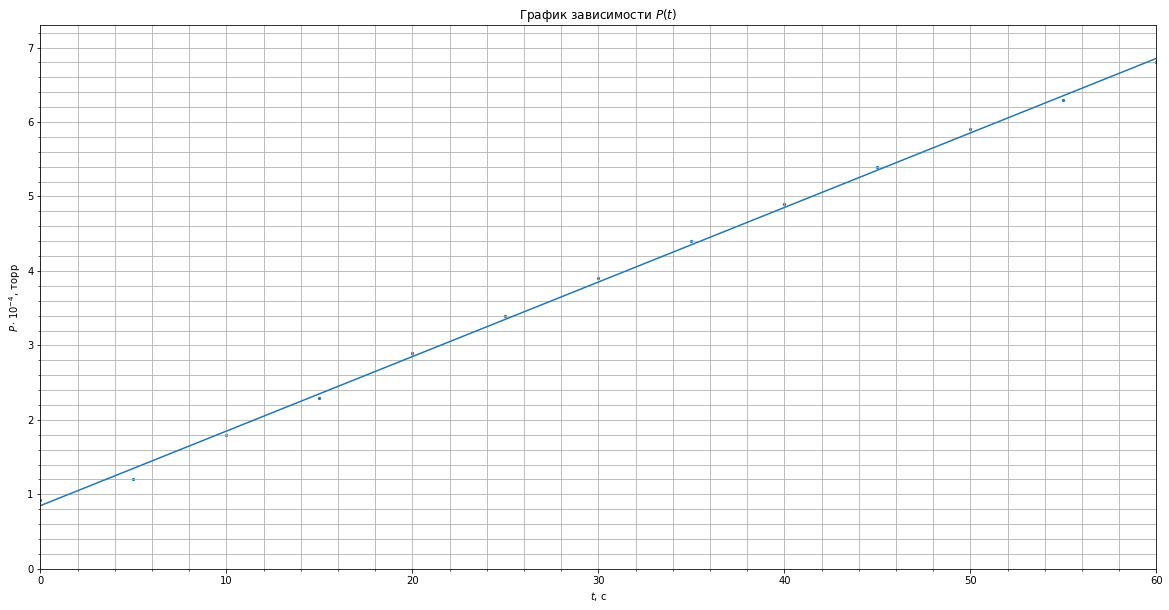
\includegraphics[scale=0.43]{graphup2}
		\caption{Ухудшение вакуума 2}
		\label{graphup2}
	\end{figure}

	\begin{figure}[h!]
		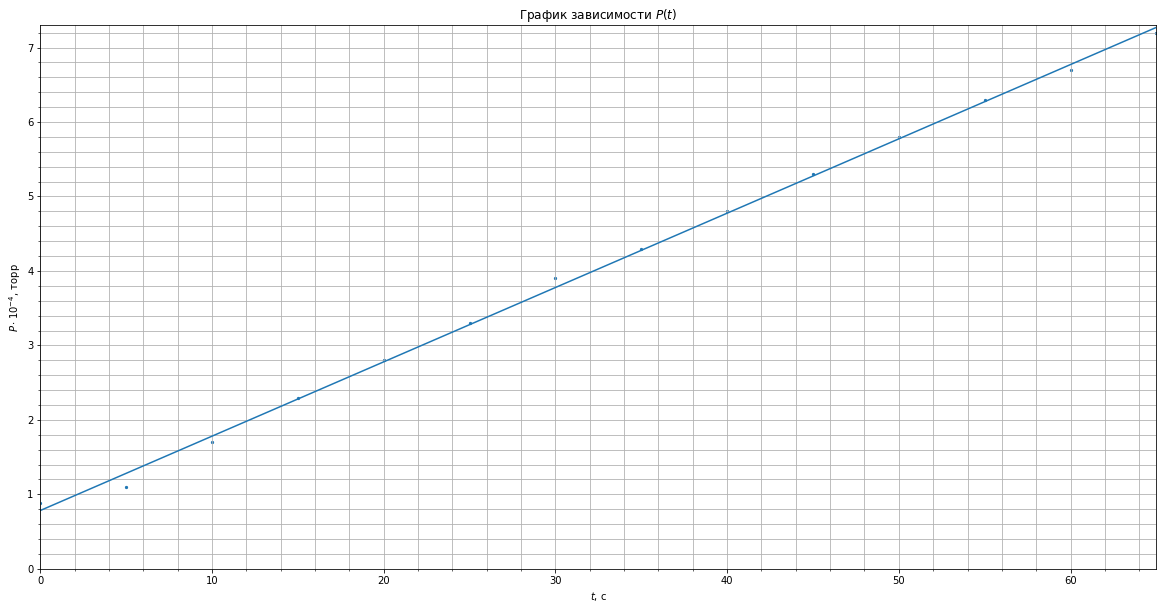
\includegraphics[scale=0.43]{graphup3}
		\caption{Ухудшение вакуума 3}
		\label{graphup3}
	\end{figure}

	\begin{figure}[h!]
		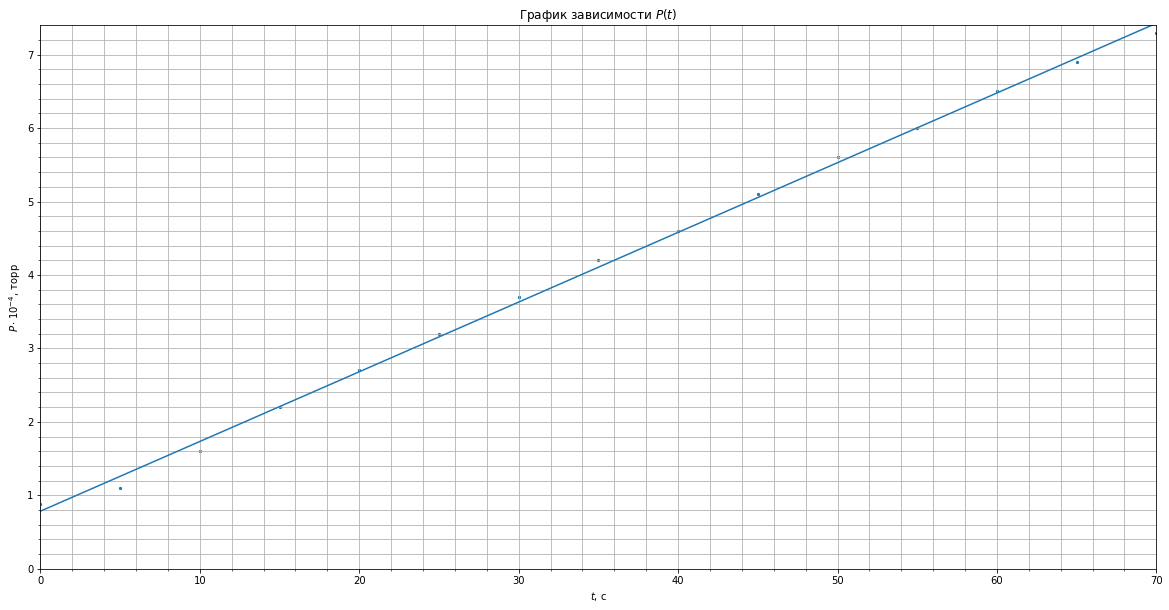
\includegraphics[scale=0.43]{graphup4}
		\caption{Ухудшение вакуума 4}
		\label{graphup4}
	\end{figure}
	
	
	
	
	
\end{document}
